\chapter{Design}

\section{Overall System Design}

\subsection{Short description of the main parts of the system}

\begin{itemize}
\item Log In Window
\item Main Database Interface
\item Adding/Removing/Editing Customers and Entries
\item Calender Interface
\item Changing Password
\item Search Window
\end{itemize}

\

Log In Window
\begin{itemize}
    \item A window is displayed which prompts the user to input their ID and password.
    \item Checks the entered valiues with the database to identify whether the user's credentials are correct.
    \item Once a correct set of values are entered, the user will be granted access to the database.
    \item A link will be at the bottom which says "Forgotten password?". This can be clicked on and then the user wil be prompted for the email address, and the corresponding password for the email address entered will be sent to that email.
    \item If there is no record of an email and password then the user will be prompted to create one for their corresponding email.
\end{itemize}

\
  
Main Database Interface
\begin{itemize}
    \item This will be the "home" interface.
    \item A view of the Customer details in the database will be available.
    \item The user can select an author from the basic view of the database, and click view
    \item A user interface is presented with a set of options which are: View, Search Database, Add Entry, Remove an Entry, Edit an Entry, Change Password, and Log out.
    \item Clicking the Search Database Button will prompt a seperate interface to open, and shows details which can be used to search for specific items in the database.

\end{itemize}

\
View Screen
\begin{itemize}
    \item Clicking view after having selected an customer will open a new window which will show a more in depth view of it. It will show the books that have been published with them.
    \item There will be buttons to expand on certain fields, including Royalties, Publishing Invoices and Book Invoices. These will show in new windows. If the user has clicked on Royalties, they have the option to click on Royalties Items on the following screen, where they can see breakdown of it. If they have clicked on Book Invoices, they can click on the Book Invoice Items on the following screen to see a breakdown of these too.
    \item Customers can be searched for quickly using their AuthorID on this screen.
\end{itemize}

\

Adding/Removing/Editing Customers and Entries
\begin{itemize}
    \item Clicking the Add Entry Button will prompt a seperate interface to open, and contains a layout of entry boxes for required fields for entering details about the customer. After this, the user can click on the customer's new record from the menu and click edit or a book/royalties/royalty items/book invoice/book invoice items/publication invoice, dependent on which has been selected. An existing customer can be selected using the search function.
    \item If a customer already exists, and details are needed to be edited or deleted, a search can be conducted to find that customer.
    \item Clicking the Remove Entry Button will prompt a seperate interface to open, which contains a view of the database, consisting of all the customers. Three search boxes can be used for searching for their forename, surname or AuthorID. If an entry was selected beforehand, then upon clicking Remove Entry, The user will be prompted for confirmation, then asked to enter their password. 
    \item Clicking the Edit Entry button will prompt a seperate interface to open, and will contain a view of the database. An entry can be searched for using the search, selected, and once the user clicks "Edit", the user will be prompted with a text box, asking for the user to enter text. Upon confirming what the user wants to enter, they are required to enter their password. This will then be saved. If a customer entry was selected before hand, a new window for adding entries will open first upon clicking Edit Entry, and the data about the customers will be in the fields already, ready for editing. Then, the data can be edited and saved, and the user will be prompted for confirmation then asked to enter their password.
\end{itemize}

\

Changing Password
\begin{itemize}
    \item An interface will open, which will prompt the user to enter their Email, Old Password, and Dhen the new password twice for confirmation.
    \item Once this has been confirmed, the interface will close, resorting back to the log in window.
\end{itemize}

\

Search Window
\begin{itemize}
    \item Clicking the Search Database Button will open a seperate interface, which contains a set of fields that the user can use to search the database by.
    \item Once the Search Button is clicked, a list of all the data entries that match the search criteria will come up in a list in the Main Window.
    \item The search can be refined by searching again, and an item can be selected from the search results.
\end{itemize}

\subsection{System flowcharts showing an overview of the complete system}

The following is a flowchart representing a summary of the complete system.

\begin{figure}[H]
    \caption{Flowchart 1} \label{Flowchart_1.pdf}
    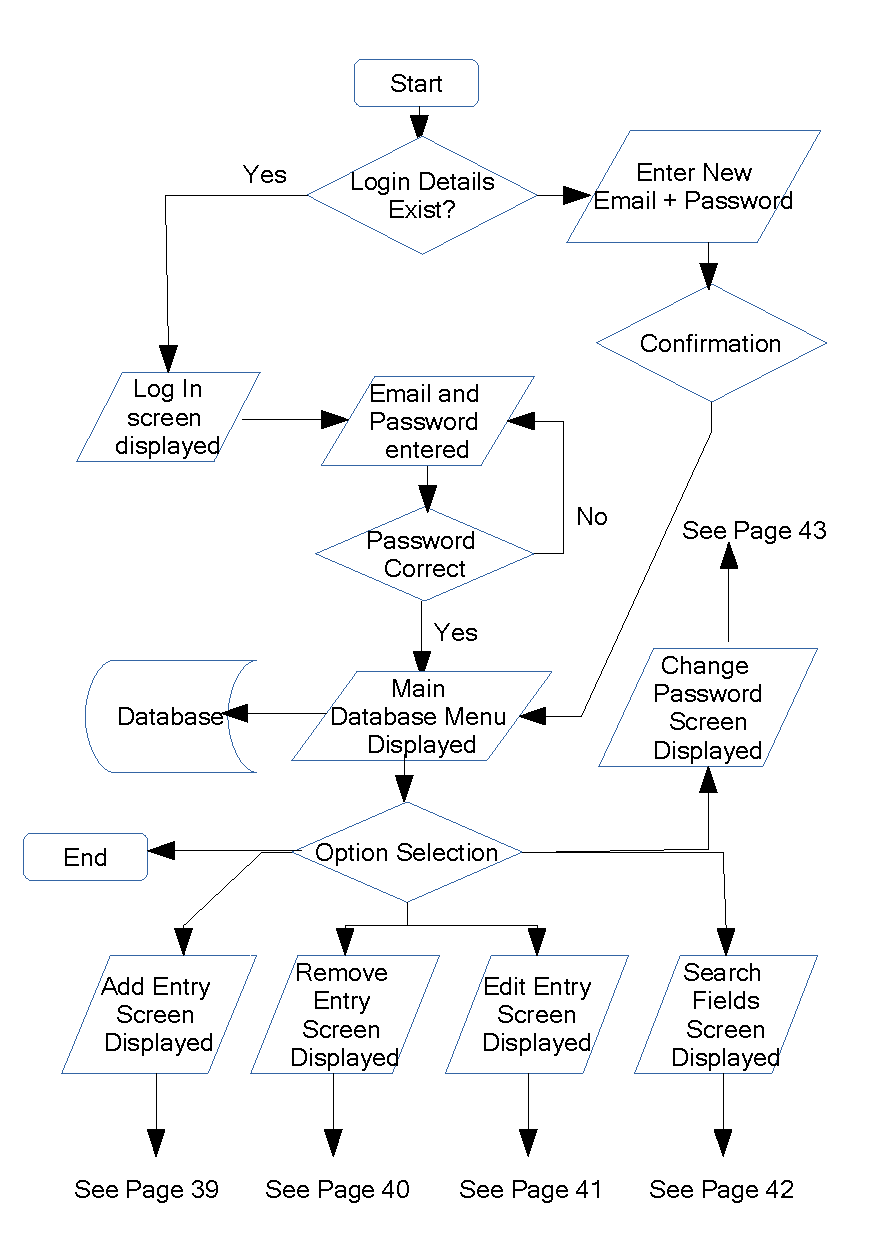
\includegraphics[width=\textwidth]{./Design/Flowcharts/Flowchart_1.pdf}
\end{figure}

\begin{figure}[H]
    \caption{Flowchart 2} \label{Flowchart_2.pdf}
    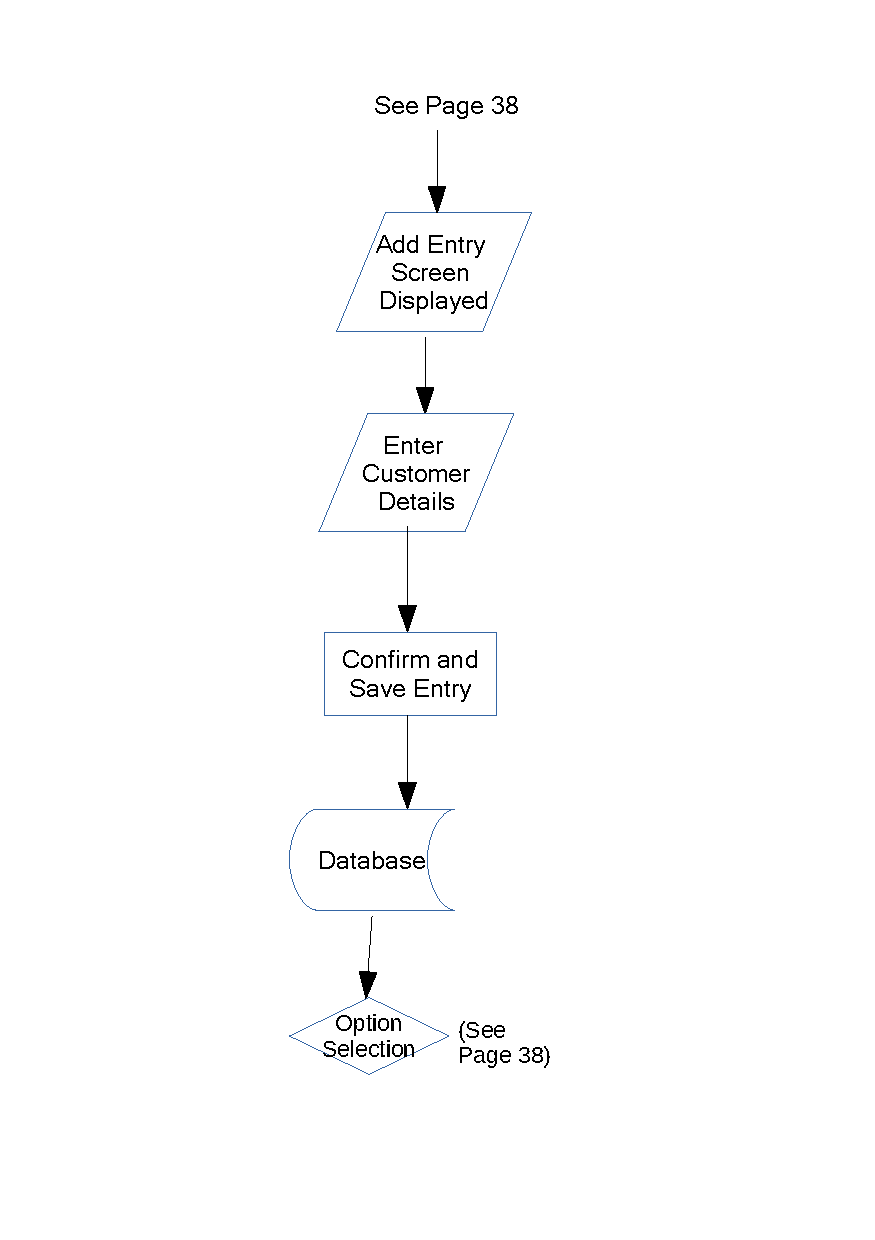
\includegraphics[width=\textwidth]{./Design/Flowcharts/Flowchart_2.pdf}
\end{figure}

\begin{figure}[H]
    \caption{Flowchart 3} \label{Flowchart_3.pdf}
    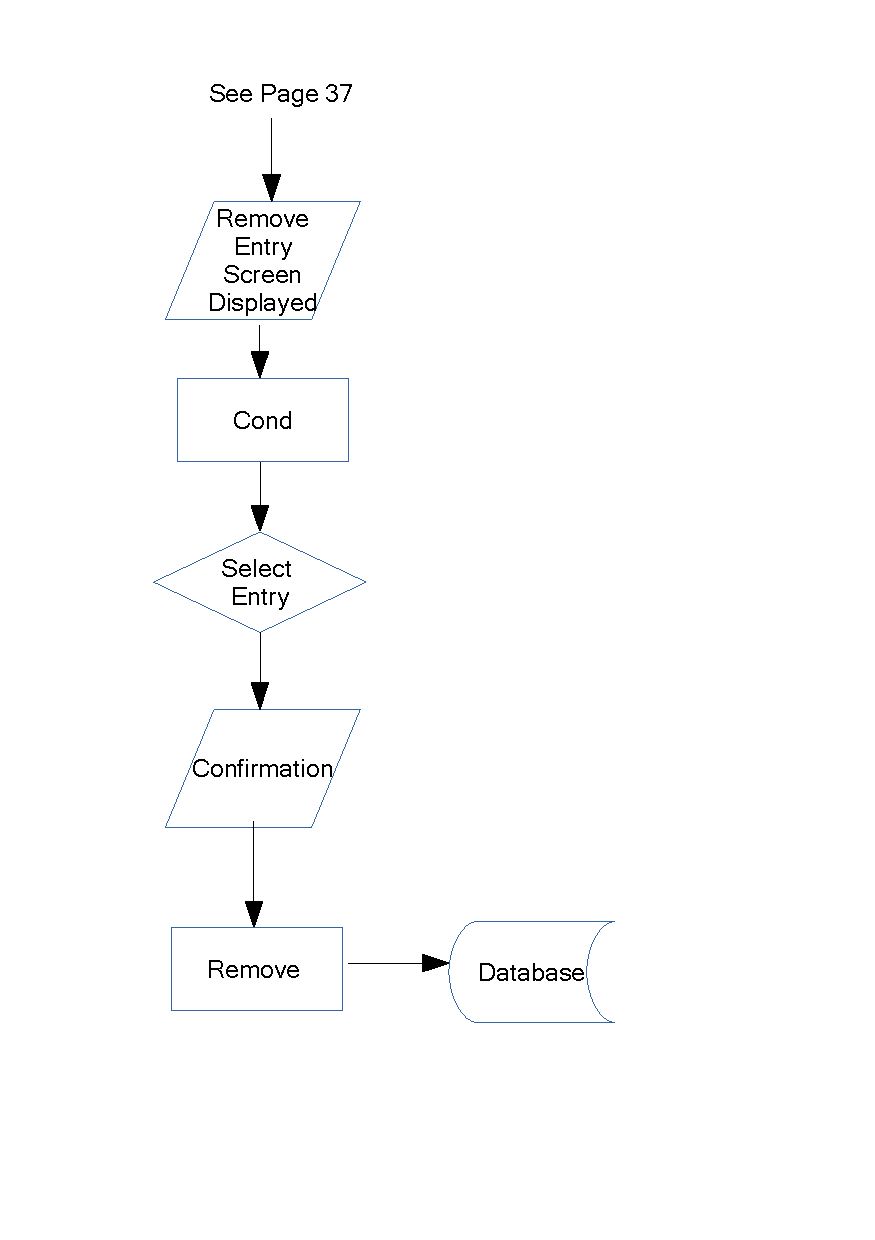
\includegraphics[width=\textwidth]{./Design/Flowcharts/Flowchart_3.pdf}
\end{figure}

\begin{figure}[H]
    \caption{Flowchart 4} \label{Flowchart_4.pdf}
    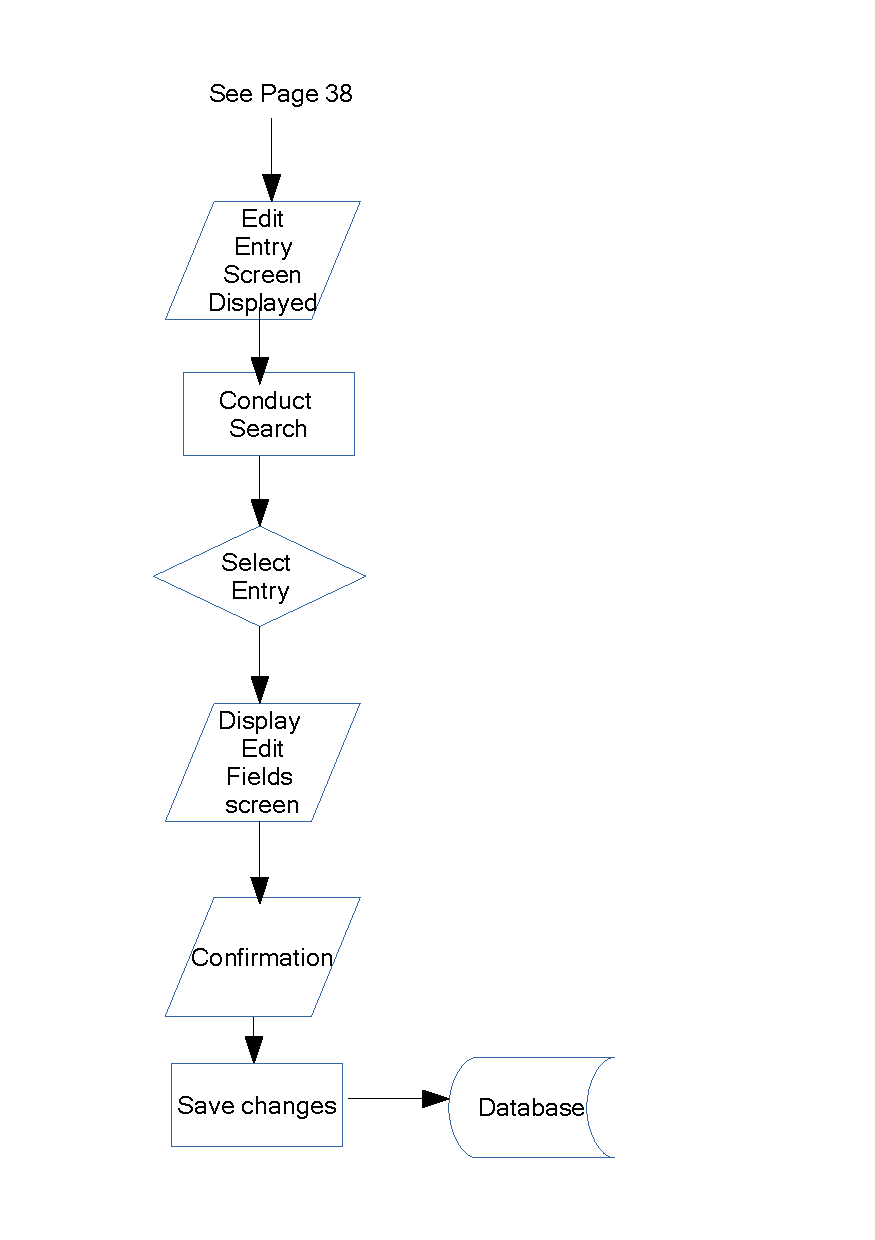
\includegraphics[width=\textwidth]{./Design/Flowcharts/Flowchart_4.pdf}
\end{figure}

\begin{figure}[H]
    \caption{Flowchart 5} \label{Flowchart_5.pdf}
    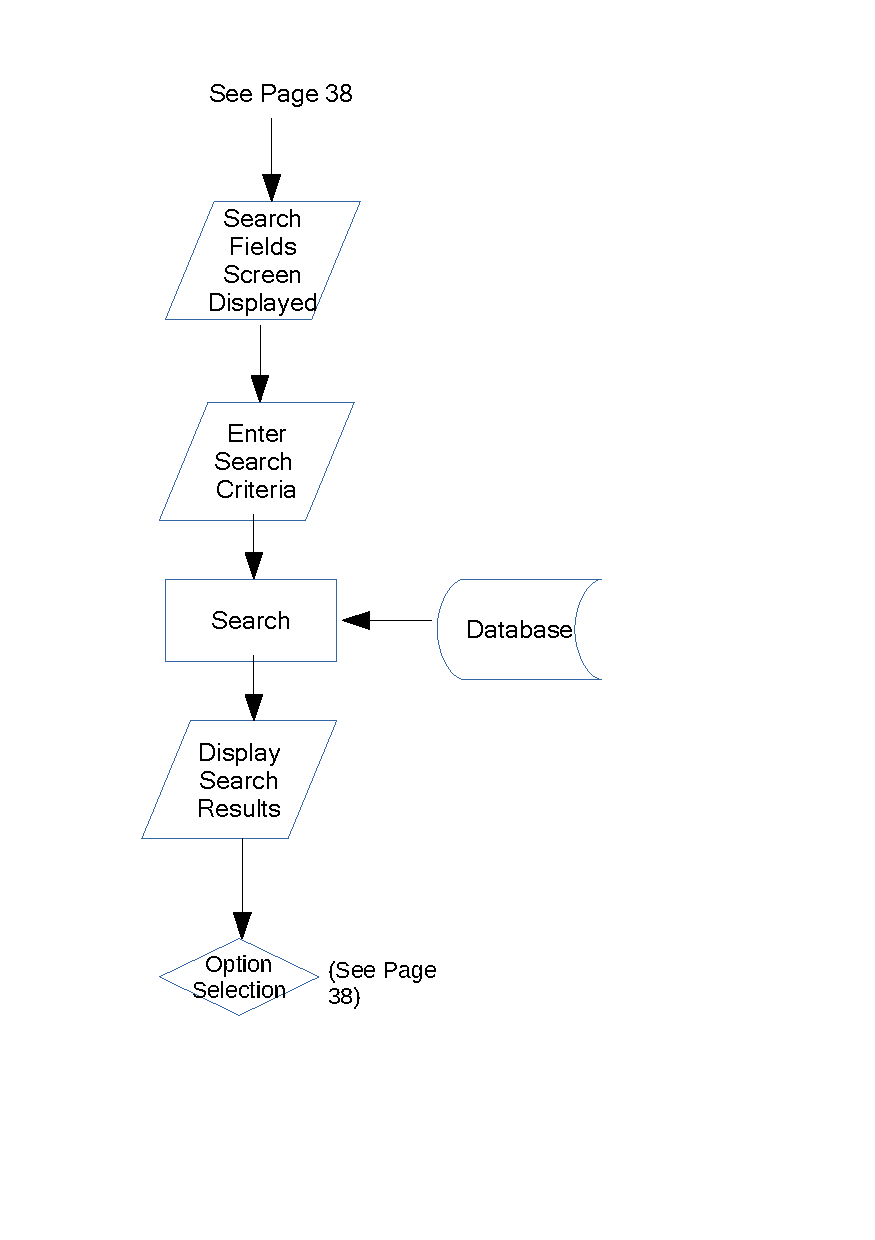
\includegraphics[width=\textwidth]{./Design/Flowcharts/Flowchart_5.pdf}
\end{figure}

\begin{figure}[H]
    \caption{Flowchart 6} \label{Flowchart_6.pdf}
    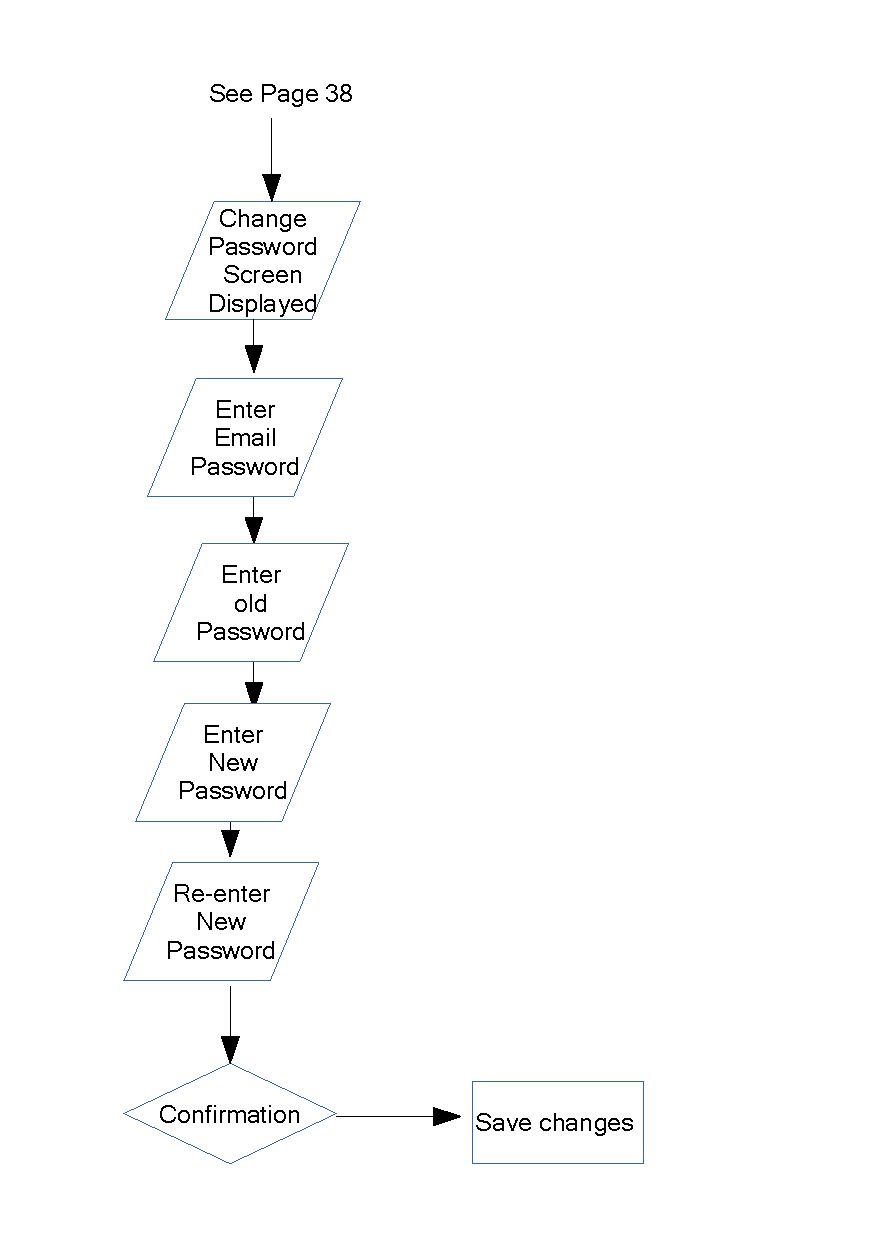
\includegraphics[width=\textwidth]{./Design/Flowcharts/Flowchart_6.pdf}
\end{figure}


\section{User Interface Designs}

\begin{figure}[H]
    \caption{Login Screen and Main Menu} \label{Login_Screen_and_Main_Menu.pdf}
    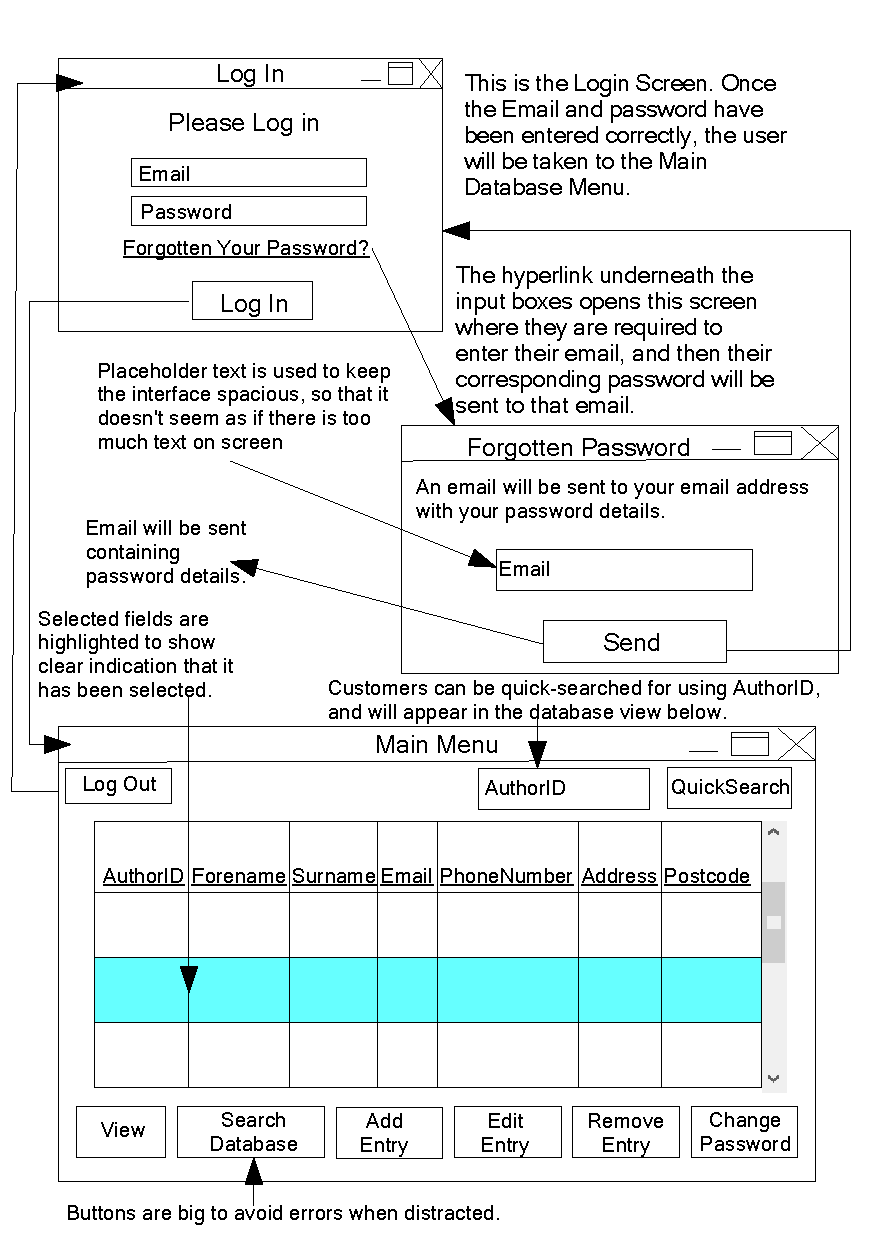
\includegraphics[width=\textwidth]{./Design/UserInterfaceDesign/Login_Screen_and_Main_Menu.pdf}
\end{figure}

\begin{figure}[H]
    \caption{View Menu and Royalties} \label{View_Menu_and_Royalties.pdf}
    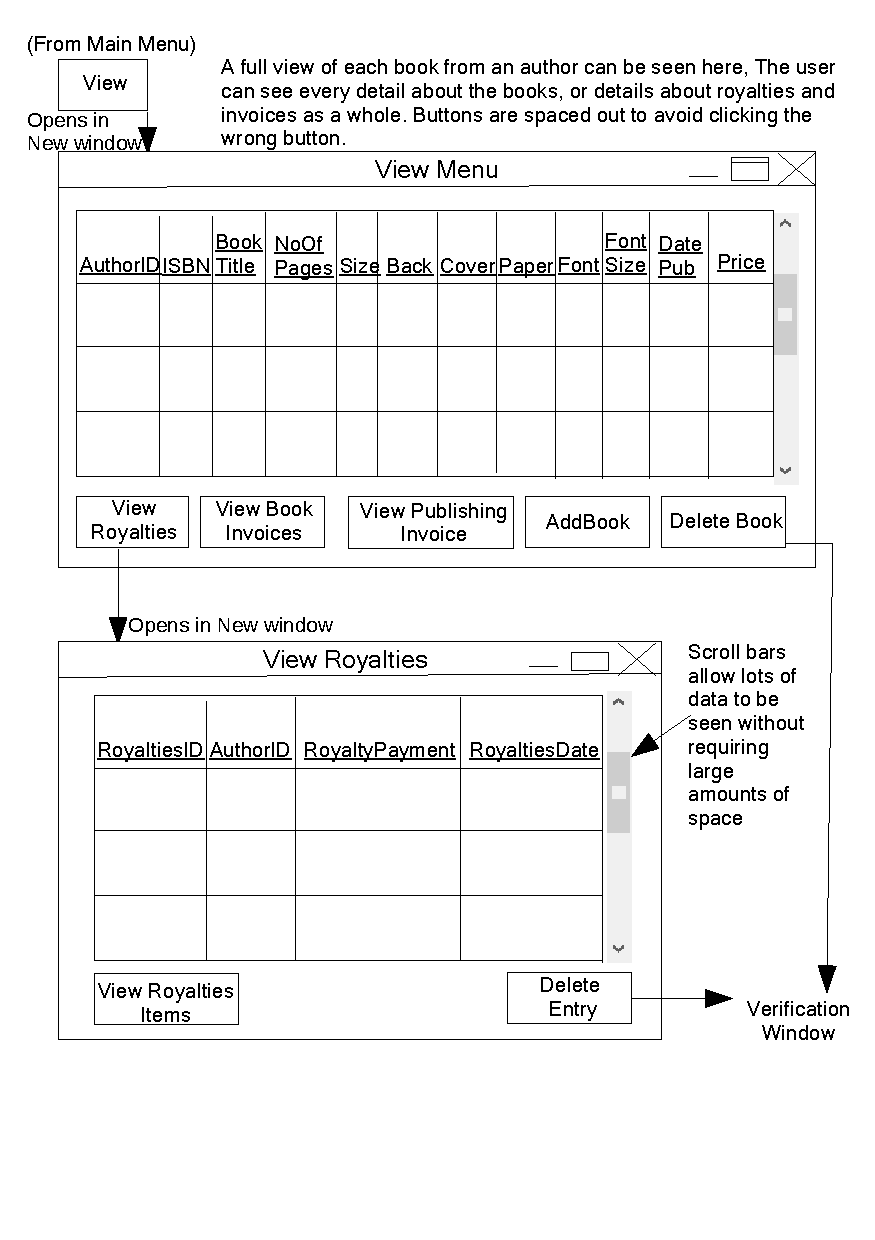
\includegraphics[width=\textwidth]{./Design/UserInterfaceDesign/View_Menu_and_Royalties.pdf}
\end{figure}

\begin{figure}[H]
    \caption{RoyaltiesItems and BookInvoice and Items} \label{RoyaltiesItems_and_BookInvoice_and_Items.pdf}
    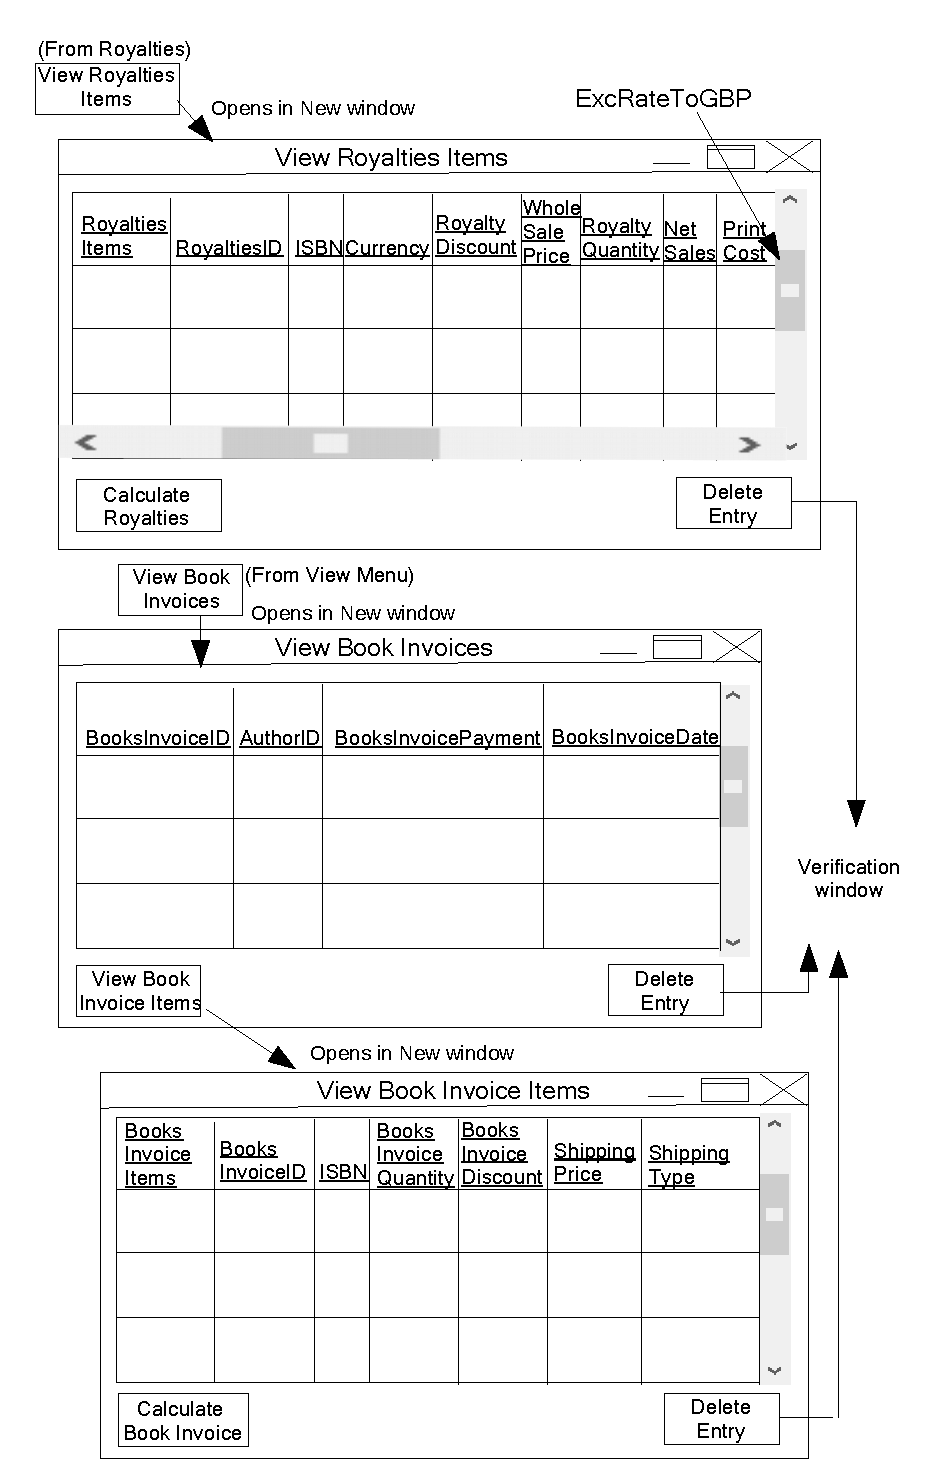
\includegraphics[width=\textwidth]{./Design/UserInterfaceDesign/RoyaltiesItems_and_BookInvoice_and_Items.pdf}
\end{figure}

\begin{figure}[H]
    \caption{Publishing Invoice and Adding Entries} \label{PubInvoice_and_Add_Entry.pdf}
    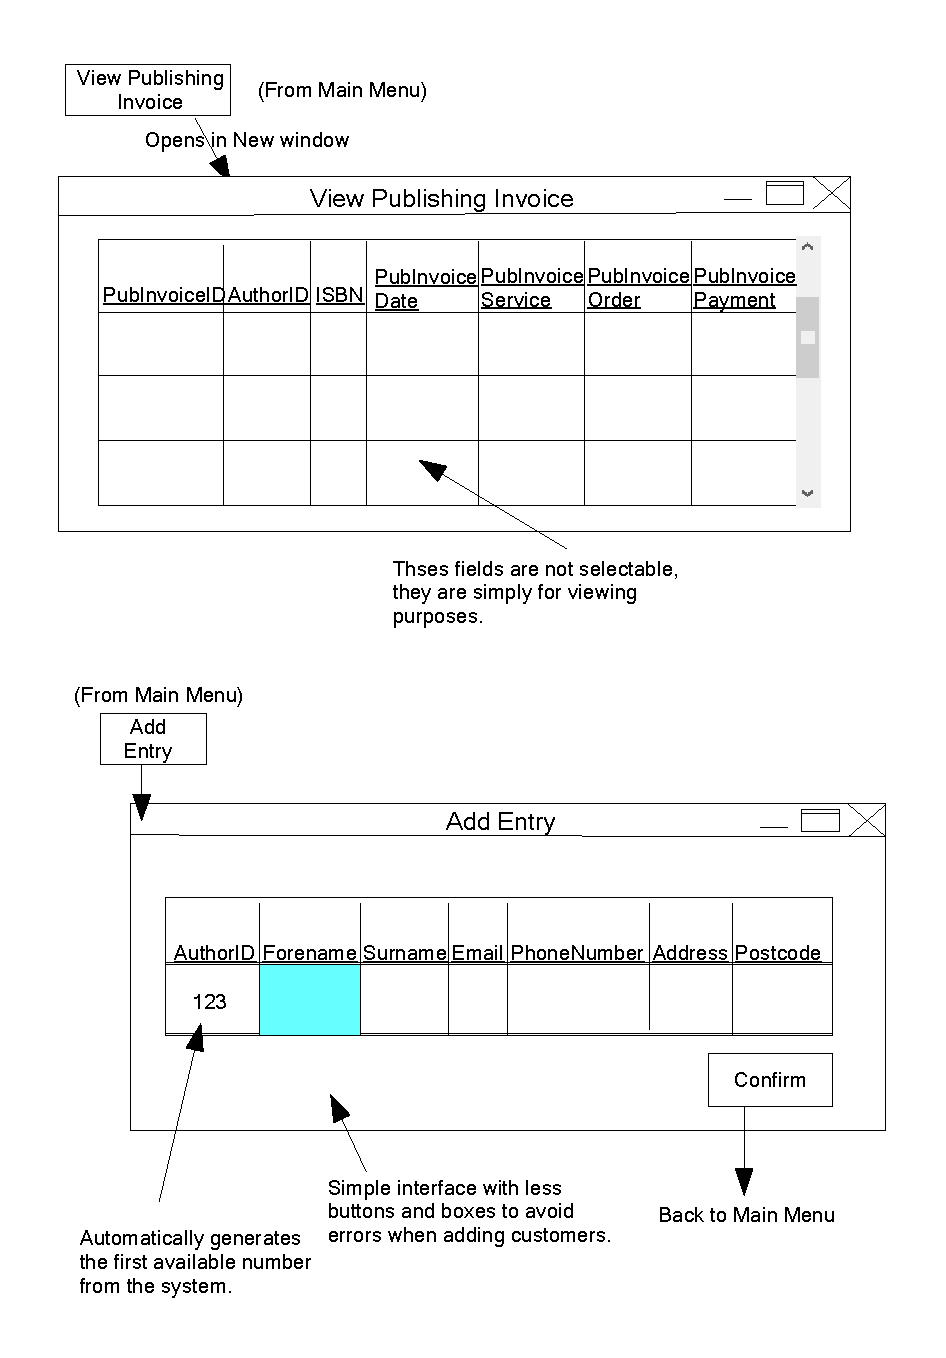
\includegraphics[width=\textwidth]{./Design/UserInterfaceDesign/PubInvoice_and_Add_Entry.pdf}
\end{figure}

\begin{figure}[H]
    \caption{Search} \label{Search.pdf}
    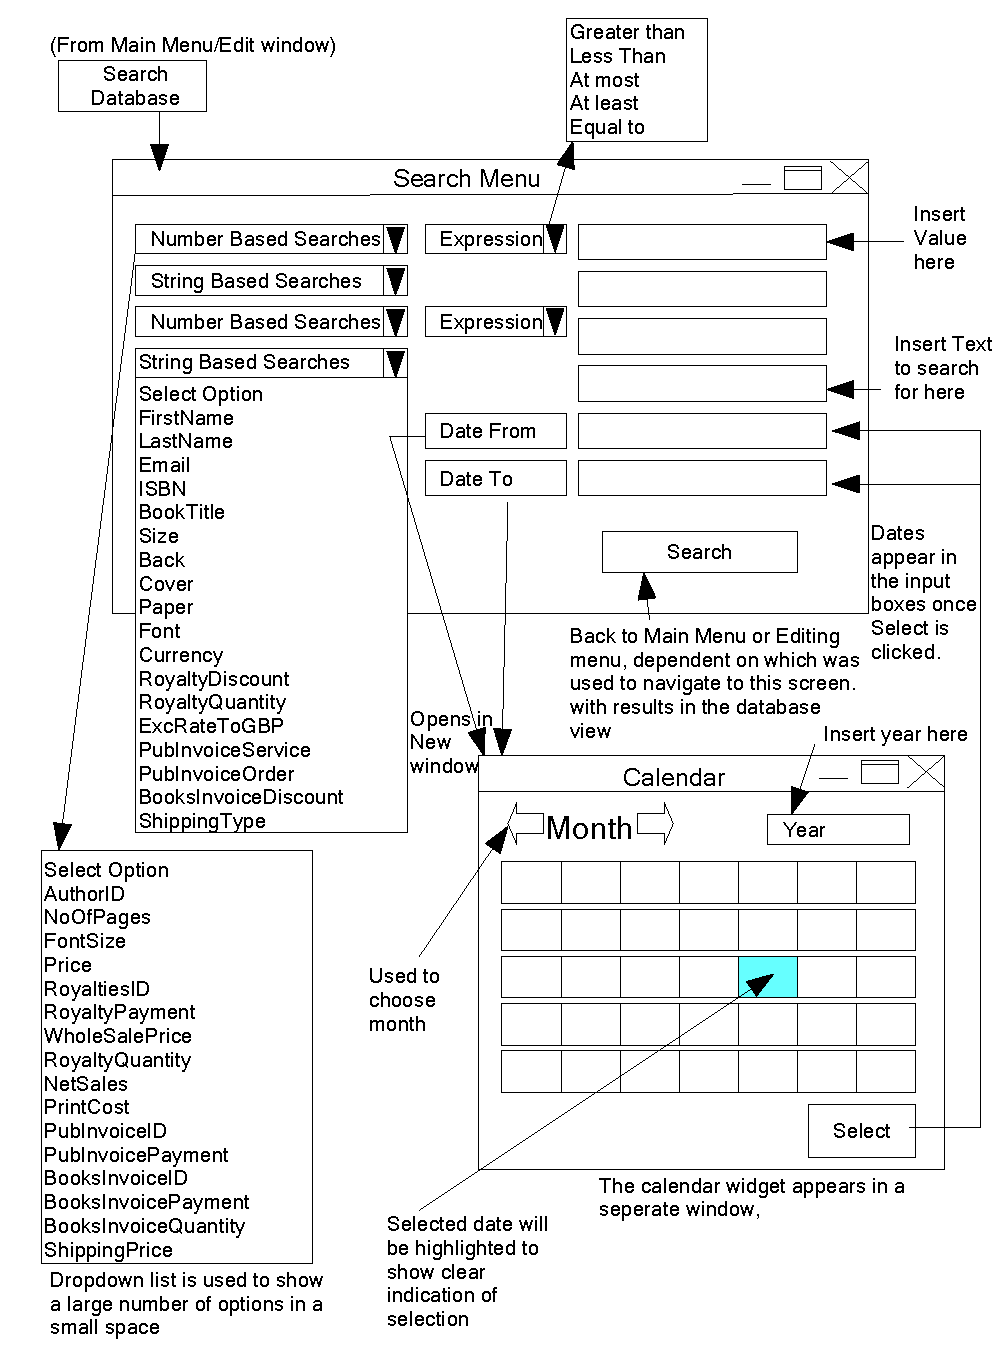
\includegraphics[width=\textwidth]{./Design/UserInterfaceDesign/Search.pdf}
\end{figure}

\begin{figure}[H]
    \caption{Editing Screens} \label{Editing_Screens.pdf}
    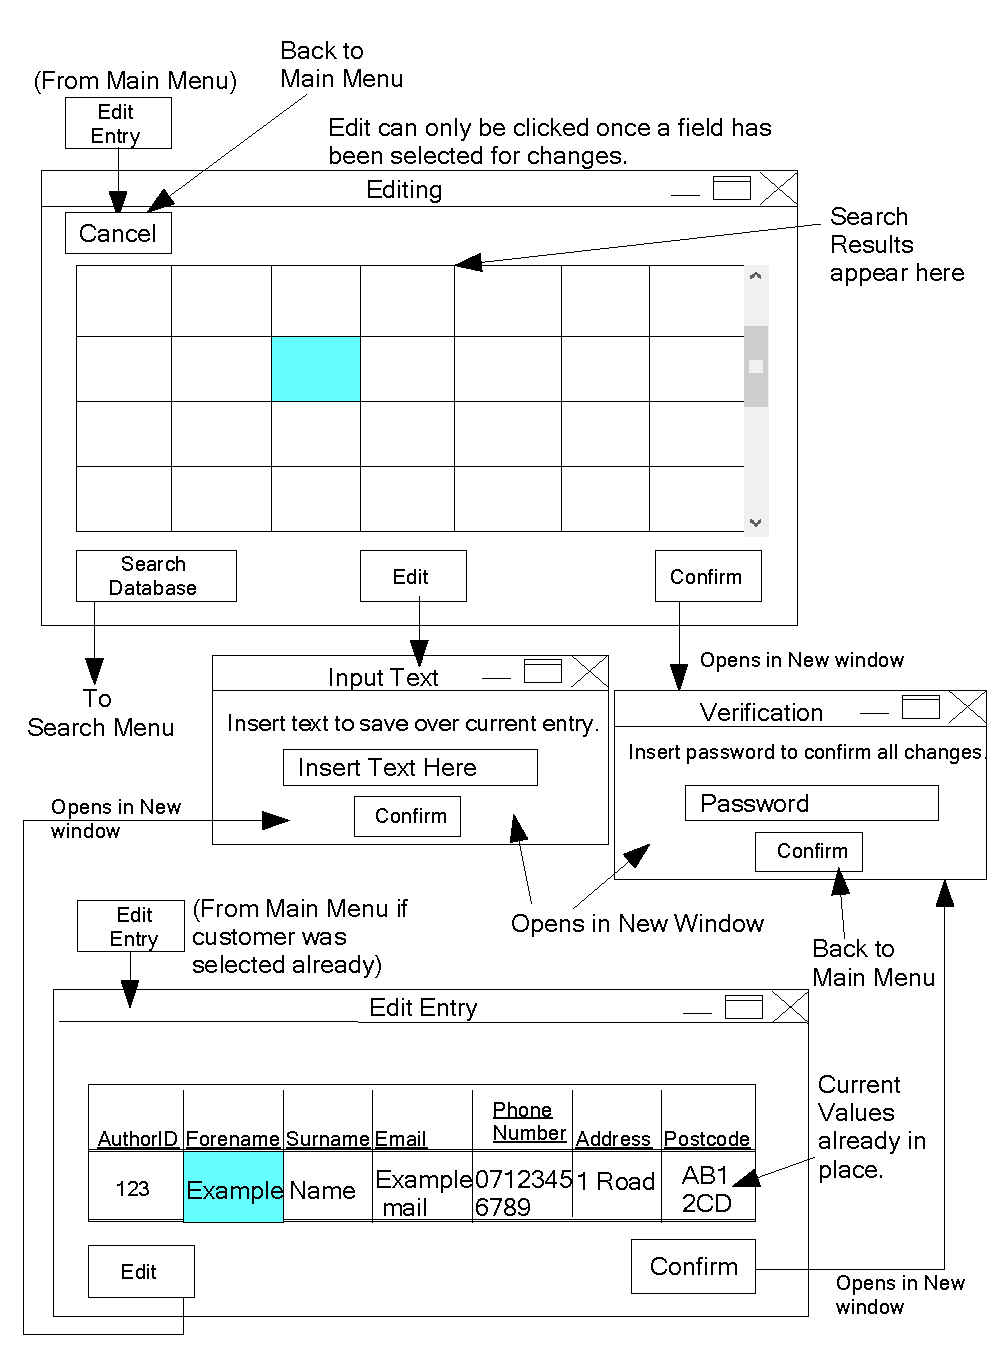
\includegraphics[width=\textwidth]{./Design/UserInterfaceDesign/Editing_Screens.pdf}
\end{figure}

\begin{figure}[H]
    \caption{Remove Entry and Change Password} \label{Remove_Entry_and_Change_Password.pdf}
    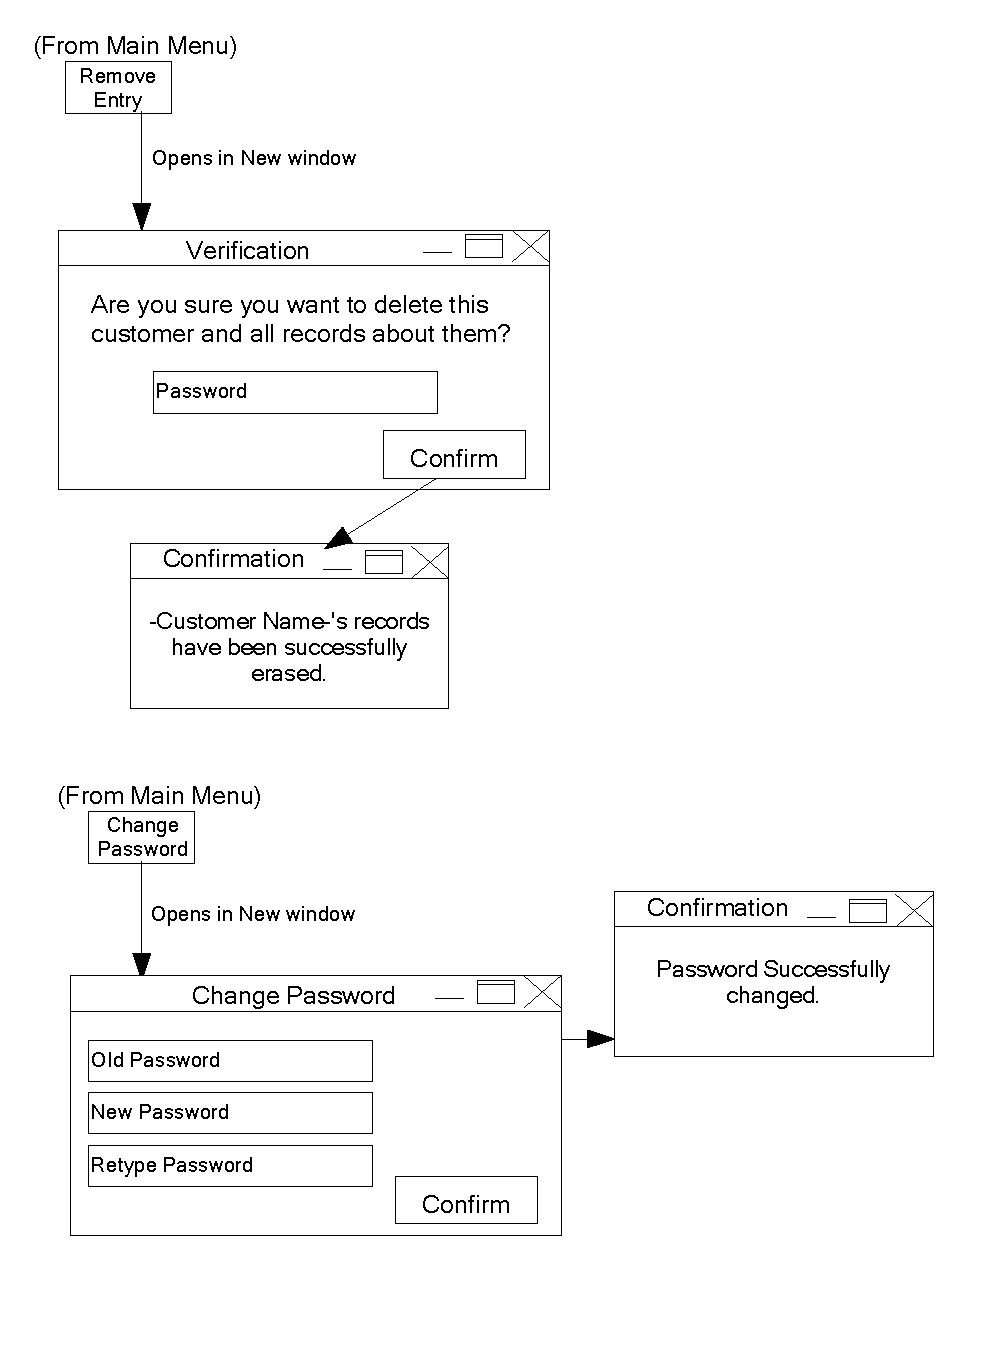
\includegraphics[width=\textwidth]{./Design/UserInterfaceDesign/Remove_Entry_and_Change_Password.pdf}
\end{figure}


\section{Hardware Specification}

The system needs to be able to run on a laptop with a 1366 x 768, 16:9 aspect ratio screen which runs on Windows 8. This is imperative to the size of the application I will be creating because it must fit on the given screen size and can't be resizable. A mouse or touchpad will be used for navigational purposes, and for confirmation of entries. Also, a keyboard will be used for inputting information into fields for entering and editing information. All the data used by the program and its database will be held on a local hard drive, and a display is needed for the outputs of the program.
%
%\section{Program Structure}
%
%\subsection{Top-down design structure charts}
%
%\subsection{Algorithms in pseudo-code for each data transformation process}
%
%\subsection{Object Diagrams}
%
%\subsection{Class Definitions}
%
%\section{Prototyping}
%
%\section{Definition of Data Requirements}
%
%\subsection{Identification of all data input items}
%
%\subsection{Identification of all data output items}
%
%\subsection{Explanation of how data output items are generated}
%
%\subsection{Data Dictionary}
%
%\subsection{Identification of appropriate storage media}


\newpage

\section{Database Design}

\subsection{Normalisation}
 
\subsubsection{ER Diagrams}


\begin{figure}[H]
    \caption{ER Diagram} \label{ER_Diagram.pdf}
    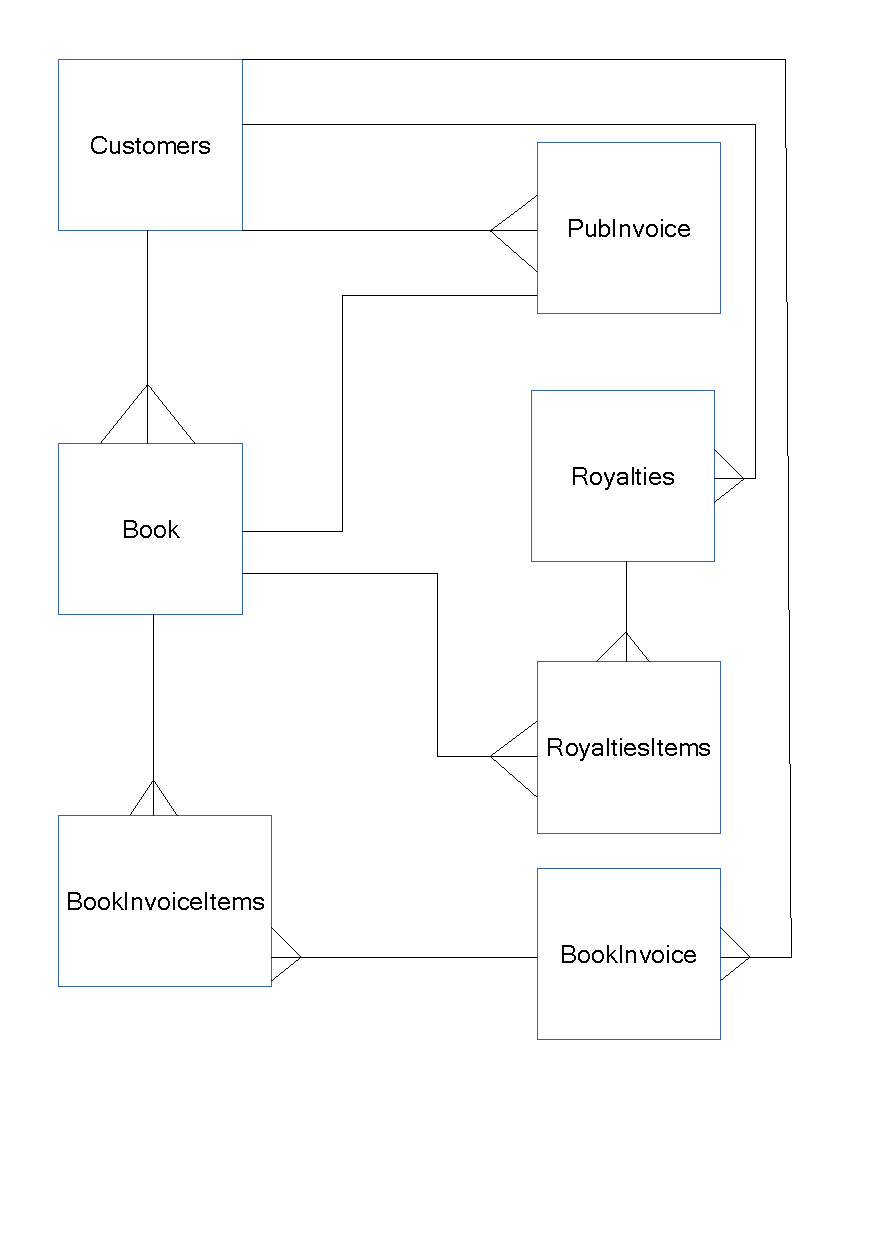
\includegraphics[width=\textwidth]{./Design/ER_Diagram.pdf}
\end{figure}


\subsubsection{Entity Descriptions}

Customer(\underline{Author ID}, FirstName, LastName, Email, Address, Postcode, Phone Number)

Invoice(\underline{InvoicePayment}, \underline{InvoiceDate}, \emph{ISBN}, \emph{AuthorID}, InvoiceQuantity, InvoiceDiscount, ShippingPrice, ShippingType)

Royalties(\underline{RoyaltyPayment}, \underline{RoyaltiesDate}, \emph{ISBN}, \emph{AuthorID}, RoyaltyDiscount, WholeSalePrice, RoyaltyQuantity, NetSales, PrintCost)

Book(\underline{ISBN}, \emph{AuthorID}, Book Title, NoOfPages, Size, Cover, Paper, Back, Paper, Font, FontSize, DatePublished, Price)

\subsubsection{UNF to 3NF}

Key:

\textbf{Bold Font} = Primary Key

\emph{Italics} = Foreign Key

Each Column represents a new group.

\newpage
First of all, I have started with the data in its unnormalised form.

\begin{tabular}{|p{3.5cm}|}
    \hline
    FirstName \\
    LastName \\
    Email \\
    PhoneNumber \\
    Address \\
    PostCode \\
    AuthorID \\
    ISBN \\
    BookTitle \\
    NoOfPages \\
    Size \\
    Back \\
    Cover \\
    Paper \\
    Font \\
    FontSize \\
    DatePublished \\
    Price \\
    RoyaltiesID \\
    RoyaltiesItems \\
    Currency \\
    RoyaltyPayment \\
    RoyaltiesDate \\
    RoyaltyDiscount \\
    WholeSalePrice \\
    RoyaltyQuantity \\
    NetSales \\
    PrintCost \\
    ExcRateToGBP \\
    PubInvoiceID \\
    PubInvoicePayment \\
    PubInvoiceDate \\
    PubInvoiceService \\
    PubInvoiceOrder \\
    BooksInvoiceID \\
    BooksInvoiceItems \\
    BooksInvoicePayment
    BooksInvoiceDate \\
    BooksInvoiceDiscount \\
    BooksInvoiceQuantity \\
    ShippingType \\
    ShippingPrice \\
    \hline
\end{tabular}

\newpage
Then, I put it into the first normal form.

\begin{tabular}{|p{2.5cm}|p{3.5cm}|}
    \hline
    \textbf{AuthorID} & \textbf{ISBN} \\
    FirstName & \textbf{AuthorID} \\
    LastName & BookTitle \\
    Email & NoOfPages \\
    PhoneNumber & Size \\
    Address & Back \\
    PostCode & Cover \\
    & Paper \\
    & Font \\
    & FontSize \\
    & DatePublished\\
    & Price \\
    & RoyaltiesID \\
    & RoyaltiesItems \\
    & Currency \\
    & RoyaltyPayment \\
    & RoyaltiesDate \\
    & RoyaltyDiscount \\
    & WholeSalePrice \\
    & RoyaltyQuantity \\
    & NetSales \\
    & PrintCost \\
    & ExcRateToGBP \\
    & PubInvoiceID \\
    & PubInvoiceDate \\
    & PubInvoiceService \\
    & PubInvoiceOrder \\
    & PubInvoicePayment \\
    & BooksInvoiceID \\
    & BooksInvoiceItems \\
    & BooksInvoicePayment \\
    & BooksInvoiceDate \\
    & BooksInvoiceDiscount \\
    & BooksInvoiceQuantity \\
    & ShippingType \\
    & ShippingPrice \\
    \hline
\end{tabular}

\newpage
After that, I put it into the second normal form.

\begin{tabular}{|p{2.5cm}|p{3.5cm}|p{2.5cm}|}
    \hline
    \textbf{AuthorID} & \textbf{ISBN} & \textbf{ISBN} \\
    FirstName & \textbf{AuthorID} & BookTitle \\
    LastName & RoyaltiesID & NoOfPages \\
    Email  & Currency & Size \\
    PhoneNumber & RoyaltyPayment & Back \\
    Address & RoyaltiesDate & Cover \\
    PostCode & RoyaltyDiscount & Paper \\
    & WholeSalePrice & Font \\
    & RoyaltyQuantity & FontSize \\
    & NetSales & DatePublished \\
    & PrintCost & Price \\
    & ExcRateToGBP & \\
    & PubInvoiceID & \\
    & PubInvoiceDate & \\
    & PubInvoiceService & \\
    & PubInvoiceOrder & \\
    & PubInvoicePayment & \\
    & BooksInvoiceID & \\
    & BooksInvoiceItems & \\
    & BooksInvoicePayment & \\
    & BooksInvoiceDate & \\
    & BooksInvoiceDiscount & \\
    & BooksInvoiceQuantity & \\
    & ShippingType & \\
    & ShippingPrice & \\
    \hline
\end{tabular}

\newpage
Finally, I put the data into its third normal form.

\begin{tabular}{|p{2.5cm}|p{2.5cm}|p{2.5cm}|p{3cm}|p{3cm}|}
    \hline
    \textbf{AuthorID} & \textbf{ISBN} & \textbf{RoyaltiesID} & \textbf{RoyaltiesItems} & \textbf{PubInvoiceID} \\
    FirstName & \emph{AuthorID} & \emph{AuthorID} & \emph{RoyaltiesID} & \emph{AuthorID} \\
    LastName & BookTitle & RoyaltyPayment & \emph{ISBN} & \emph{ISBN} \\
    Email & NoOfPages & RoyaltiesDate & Currency & PubInvoiceDate \\
    PhoneNumber & Size & & RoyaltyDiscount & PubInvoiceService \\
    Address & Back & & WholeSalePrice & PubInvoiceOrder \\
    PostCode & Cover & & RoyaltyQuantity & PubInvoicePayment \\
    & Paper & & NetSales & \\
    & Font & & PrintCost & \\
    & FontSize & & ExcRateToGBP & \\
    & DatePublished & & & \\
    & Price & & & \\
    \hline
\end{tabular}

\begin{tabular}{|p{3.5cm}|p{3.5cm}|}
    \hline
    \textbf{BooksInvoiceID} & \textbf{BooksInvoiceItems} \\
    \emph{AuthorID} & \emph{BooksInvoiceID} \\
    BooksInvoicePayment & \emph{ISBN} \\
    BooksInvoiceDate & BooksInvoiceQuantity \\
    & BooksInvoiceDiscount \\
    & ShippingType \\
    & ShippingPrice \\
    \hline
\end{tabular}

\newpage

\subsection{SQL Queries}

I am using Python to format the SQL query text strings.

\begin{tabular}{|p{10cm}|p{5cm}|}
    \hline
    \textbf{SQL} & \textbf{Descriptions} \\ \hline 
     """insert into \\ Customer(FirstName, LastName, Email, PhoneNumber, Address, Postcode) values (\{0\}, \{1\}, \{2\}, \{3\}, \{4\}, \{5\}) \\ """.format(FirstName, LastName, Email, PhoneNumber, Address, Postcode) & An example of an SQL statement which adds customer records to the database. Here, it is entering a new customer record with the attributes: FirstName, LastName, Email, PhoneNumber, Address and Postcode. \\ \hline
    """create table RoyaltiesItems(\\ RoyaltiesID INTEGER, \\ Currency REAL, \\ RoyaltyDiscount STRING,\\  WholeSalePrice REAL,\\ RoyaltyQuantity INTEGER,\\ NetSales REAL,\\ PrintCost REAL, \\ ExcRateToGBP STRING \\ PRIMARY KEY(RoyaltiesItems) \\ FOREIGN KEY(RoyaltiesID) REFERENCES \\ Royalties(RoyaltiesID) """ & An example of an SQL statement that creates a new table for the Royalties. There is a primary key which is RoyaltiesItems, and there is one foreign key, which is RoyaltiesID. \\ \hline 
    """select Customer.LastName, Book.BookTitle \\ from Customer, Book \\ where Price < 13.00 and \\ Back = "Paperback"  & This statement will return all the LastNames and the BookTitles from the Customer table and the Book table whose book is paperback and costs less than £13. \\ \hline
\end{tabular}

%\section{Security and Integrity of the System and Data}
%
%\subsection{Security and Integrity of Data}
%
%\subsection{System Security}
%
%\section{Validation}
%
%\section{Testing}

\begin{landscape}
\subsection{Outline Plan}

\begin{center}
    \begin{tabular}{|p{2cm}|p{5cm}|p{5cm}|p{4cm}|}
        \hline
        \textbf{Test Series} & \textbf{Purpose of Test Series} & \textbf{Testing Strategy} & \textbf{Strategy Rationale}\\ \hline
        Example & Example & Example & Example \\ \hline
    \end{tabular}
\end{center}

\subsection{Detailed Plan}

\begin{center}
    \begin{longtable}{|p{1.5cm}|p{2.5cm}|p{2.5cm}|p{2cm}|p{2cm}|p{2cm}|p{2cm}|p{2cm}|}
        \hline
        \textbf{Test Series} & \textbf{Purpose of Test} & \textbf{Test Description} & \textbf{Test Data} & \textbf{Test Data Type (Normal/ Erroneous/ Boundary)} & \textbf{Expected Result} & \textbf{Actual Result} & \textbf{Evidence}\\ \hline
        Example & Example & Example & Example & Example & Example & Example & Example \\ \hline
    \end{longtable}
\end{center}
\end{landscape}